%!TEX encoding = UTF-8 Unicode
\chapter{攻击技术}
安全界一直存在这样的争议:攻击技术的充分公开,带来的是更多的模仿,还是更有效的防范?在PC病毒发展的早期,一次病毒源码公开事件带来了史上第一次病毒数量的爆发\footnote{1987年9月,Ralf Burger在他的书\textit{Computer Viruses: a High-tech Disease}中公布了感染式病毒Vienna的反汇编代码,并详细介绍了计算机病毒的工作原理和编写方法。随后,大量模仿它的新病毒出现。},这成为前一观点支持者的论据之一。

在这个问题上,笔者的看法如下:
\begin{enumerate}
  \item 正如前言所述,在这个领域、这个时候,公开交流所带来的边界收益会比它可能带来的损失要大得多;
  \item 安全工程师要分析、检测、防御恶意代码,了解其攻击技术这一步骤是不可避免的;
  \item Peter Szor曾说\cite{art_virus}:“即使你编写了许多计算机病毒,也不能使你成为这一领域的专家。”
\end{enumerate}

因此,这一章我们将介绍对一些攻击技术的概念验证(PoC, Proof of Concept)或实际分析。
\section{重新打包}
\label{Sec:repackage}
重新打包(re-package)又称植入,是目前Android平台主要攻击方式之一。2011年3月初,Google的官方Market上出现58款被植入恶意代码DroidDream的应用程序,就是利用了这一技术。

所谓植入攻击,是指攻击者将恶意代码植入正常软件中,通过软件市场、下载站、手机论坛等途径分发给用户。用户安装后,正常使用软件而感觉不到任何异常,但附带的恶意代码已经开始运行。从概念上看,这类攻击很像PC平台的感染式病毒。但与感染式病毒不同的是,植入型攻击并无自我复制性,而是通过这种“植入”而获得伪装效果,即类似于木马。

植入型攻击是一种危险性极大的攻击手段。一份恶意代码可以植入多个正常软件,即使单个软件的传播范围不广,但移植成本几乎为零,因此可以批量植入,最终造成大范围攻击。此外,用户安装了被植入的软件后,在第一次使用软件之前,恶意代码就能通过大量系统事件(例如接听电话、收发短信、开机等)而触发开始执行,这是它与PC病毒的另一不同之处。

植入型攻击的步骤可以分为:编写攻击代码、解包正常软件、植入恶意代码、重新打包、重新签名。接下来我们逐一介绍并编码实现。
\subsection{编写攻击代码}
恶意代码为了持久有效地攻击,通常有两种意图:
\begin{enumerate}
	\item 隐蔽而不被用户察觉,以延长攻击时间,增加攻击次数和可能;
	\item 尽早运行,以快速攻击、快速获利、快速退出。
\end{enumerate}
因此它既不能影响被植入软件的正常运行,以免被用户发现;又要防止用户安装了以后不手工点击运行,因此要有自动启动的能力。我们曾介绍,Android平台上,一个软件可以有多个入口点——不同的活动、服务、广播接收器等。植入型攻击正是利用了广播接收器来自启动,并利用服务持久化攻击。

我们建立一个包名为com.example.Malware的“恶意代码”,并在其中实现名为\lstinline!SmsReceiver!的广播接收器,代码如下:
\lstinputlisting[language=Java,caption=SmsReceiver.java,label=Code:SmsReceiver]{code/SmsReceiver.java}

\lstinline!SmsReceiver!继承了Android的\lstinline!BroadcastReceiver!类,在重载的\lstinline!onReceive()!函数中,用\lstinline!Toast!弹出一个提示信息,以便后续观察是否成功运行。攻击者一般利用这一执行机会开启一个新的服务,并在服务中真正地开始恶意行为。

为了在每次收到短信时触发\lstinline!SmsReceiver!,我们在\lstinline!AndroidManifest.xml!文件中进行申明、设置intent-filter,并申请接收短信权限:
\lstinputlisting[language=XML,caption=Malware的AndroidManifest.xml, label=Code:MalwareManifest]{code/MalwareManifest.xml}
其中,第6行申请了\lstinline!RECEIVER_SMS!的权限,7到11行注册了这个BroadcastReceiver并设置了对收短信行为的intent-filter。注意我们在\lstinline!receiver!的\lstinline!android:name!属性中没有使用\lstinline!.SmsReceiver!的缩写路径,而是采用全路径,这是为后面植入所准备。

恶意代码通常设置多种常见系统事件的接收器,在它们的\lstinline!onReceive()!实现中开启一个恶意的服务。我们不演示这些行为,直接将工程编译,得到Malware.apk。
\subsection{解包正常软件}
选取一个正常软件的安装文件,例如Software.apk(package名为net.claudxiao.Software)。利用apktool工具\footnote{http://code.google.com/p/android-apktool/}将其解包:
\begin{lstlisting}[language=bash, numbers=none]
apktool d Software.apk
\end{lstlisting}
成功解包后,当前目录下会生成名为Software的目录。类似地,我们将上一节编写的Malware.apk解包,得到Malware目录。
\subsection{植入恶意代码}
我们需要使用Malware.apk中的接收器\lstinline!SmsReceiver!。因此,将apktool解包和反汇编后得到的Malware/smali/com/example/Malware/SmsReceiver.smali文件拷贝至Software目录的对应路径下,即Software/smali/com/example/Malware/SmsReceiver.smali。

接下来修改Software/AndroidManifest.xml文件,在其中添加\ref{Code:SmsReceiver}的6到11行,得到如下XML文件:
\lstinputlisting[language=XML,caption=被植入的AndroidManifest.xml, label=Code:NormalManifest]{code/NormalManifest.xml}
注意,这里\lstinline!receiver!的\lstinline!android:name!属性继续使用了全路径。
\subsection{重新打包}
使用apktool重新打包Software:
\begin{lstlisting}[language=bash, numbers=none]
apktool b Software unsigned.apk
\end{lstlisting}
在当前目录生成了名为unsigned.apk的安装包。这个包还无法安装到手机或模拟器上,因为apktool并不生成安装包的签名数据。
\subsection{重新签名}
使用Android源码编译中得到的signapk.jar工具以及用于测试的密钥testkey.pk8和testkey.x509.pem对上一步产生的unsigned.apk签名:
\begin{lstlisting}[language=bash, numbers=none]
java -jar signapk.jar testkey.x509.pem testkey.pk8 unsigned.apk infected.apk
\end{lstlisting}
这样,我们就得到了一个具有签名的被植入软件。用户使用它时,会和植入前的表现一模一样,但已经包含了一个短信事件接收器。
\subsection{攻击效果验证}
\begin{figure}[htb]
	\centering
	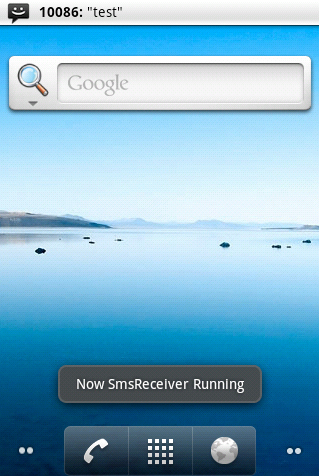
\includegraphics[width=8cm]{image/toast.jpg}
 	 \caption{植入型攻击PoC演示效果}
	 \label{Fig:Toast}
\end{figure}
将infected.apk安装到模拟器,并向模拟器发一条短信\footnote{使用ddms或者telnet工具,请参考SDK文档或Android开发书籍}。如图\ref{Fig:Toast}所示,可以看到\lstinline!Toast!的提示消息已经弹出,也就是说在收到短信的同时,我们植入的代码已经运行起来了。
\section{代码混淆}
\section{类的动态加载}
